\chapter{MRI Simulation}
\label{chapterlabel3}

Magnetic Resonance Imaging is an imaging technique that is widely used today in clinics and medical research facilities to aid the understanding of how the human body works. It has many applications in the biomedical sciences such as the study of the human anatomy, pathology and even function. 

In contrast to other well established imaging modalities, MRI is incredibly versatile as it is capable of displaying high quality images of any orientation through the human body without the need for the patient to be uncomfortable or move. Furthermore, MRI is based on non-ionizing radiation and it is classified as a non-invasive modality achieving great soft tissue resolution. Its applications span from neuroimaging, heart imaging, angiography, to spectroscopy, diffusion, perfusion imaging, and many others.

The entire process of an MRI scan, from proton to picture, is incredibly complex and requires a great understanding of the underlying physics. Nevertheless, from a high level perspective, a clinical examination using an MR scanner is made up of a few important steps. First, the object that is being imaged and which consists of billions of protons randomly oriented inside the tissue is needed. This object can be an MRI phantom, a tissue sample or an organ of interest. Second, the actual hardware of the MRI scanner is needed in order to create the strong magnetic field used to orient the spins magnetic moments. In addition, gradient coils are needed in order to spatially resolve the spins positions. Also, radio frequency coils are used to transmit rf pulses and to receive the signal generated by the sample. Third, a recipe for how to use the scanner in order to acquire images of desired contrast is needed. Parameters such as RF flip angle, the repetition time and the echo time can be set by the clinician. 

These three main building blocks are necessary in order to produce the signal. Once the signal is generated, it can be collected and sampled in order to be stored in a matrix form, called k-space. When the whole of k-space has been covered, the reconstruction process (a 2D Fast Fourier transform is applied) can start and the final image is obtained. This pipeline is visually presented in Figure~\ref{fig:mriscan}. 

\begin{figure}[H]
    \centering
    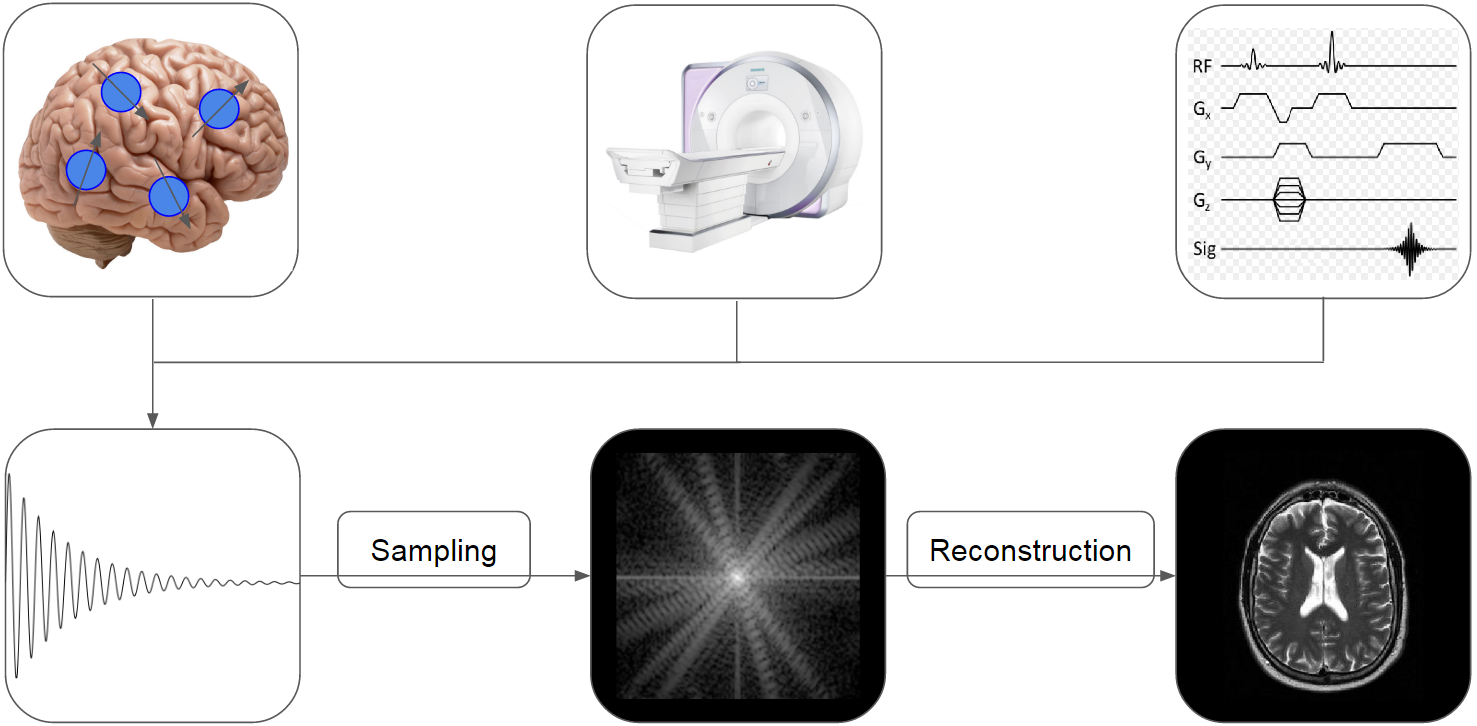
\includegraphics[width=1\textwidth,keepaspectratio]{mriscan}
    \caption{The MRI scan pipeline}
    \label{fig:mriscan}
\end{figure}

However, it is not the full story. A high quality image cannot be achieved unless a few criteria are met. First, the object being imaged has to be completely stationary or motion artefacts will appear in the final image. Even if the patient manages not to move, there is always some movement caused by pulsatile flow or respiration. Second, the scanner's electronic components have an inherent level of noise which will appear in the images. Third, air-tissue boundaries create inhomogeneities in the main magnetic field which will cause distortions in the final images. Fourth, good contrast between the tissue types that are being imaged is achieved when the right combination of sequence parameters is found. All in all, these are just a few of the problems that lead to imperfect images and therefore MRI images need to be corrected and MR parameters need to be mingled with in order to have the best results. 

Under these circumstances, 
the need for MRI simulation was born. There are at least three main reasons for creating an accurate and realistic MR simulator and they can be summarised as follows. First, MR physicists and clinicians need to learn how to use the scanner in order to gain experience. By using an actual MR scanner they would also need a patient or a good phantom to be able to learn how to program a sequence. Moreover, trying out new sequences could take time and scanners are precious medical devices that are needed by patients throughout the year. Second, there is always place for improvement when it comes to contrast-to-noise ratio in MR images. For example, enhancing a pathology in an image requires a fine tuning of the sequence parameters and this process is too time consuming for it to be practiced on a real person and a real MR scanner. Third, there is a large body of research concerning the correction of different imaging artefacts that appear in MR images. All these algorithms require ground truth to be tested and validated against. An MRI simulator can provide this ground truth. In conclusion, simulating the MRI process from object to final image is important and needed in the biomedical sciences.

That being said, the following subsections will be focused on how the ideal simulator should look, what approaches different MRI simulators have taken up until today and how they fit inside the ideal picture and, finally, a review of the active simulators will be provided.

%%%%%%%%%%%%%%%%%%%%%%%%%%
\section{Ideal Simulator}
We have discussed so far about the importance of MRI and the benefits of having an MRI simulator. In this subsection the focus will be on an ideal MRI simulator. As can be expected with any type of physics oriented simulation, the best approach is to emulate the reality as close as possible. That being said, the pipeline presented before is changed to accommodate simulated objects, simulated hardware and simulated sequences. This can be seen in Figure~\ref{fig:mrisimscan}. Now, instead of a real object, we have tissue samples, description of motion patterns and tissue specific parameters. Also, instead of a scanner, we have the scanner specifications being simulated as close to reality as possible and, instead of a real sequence, the sequence specifications are provided and simulated.

\begin{figure}[H]
    \centering
    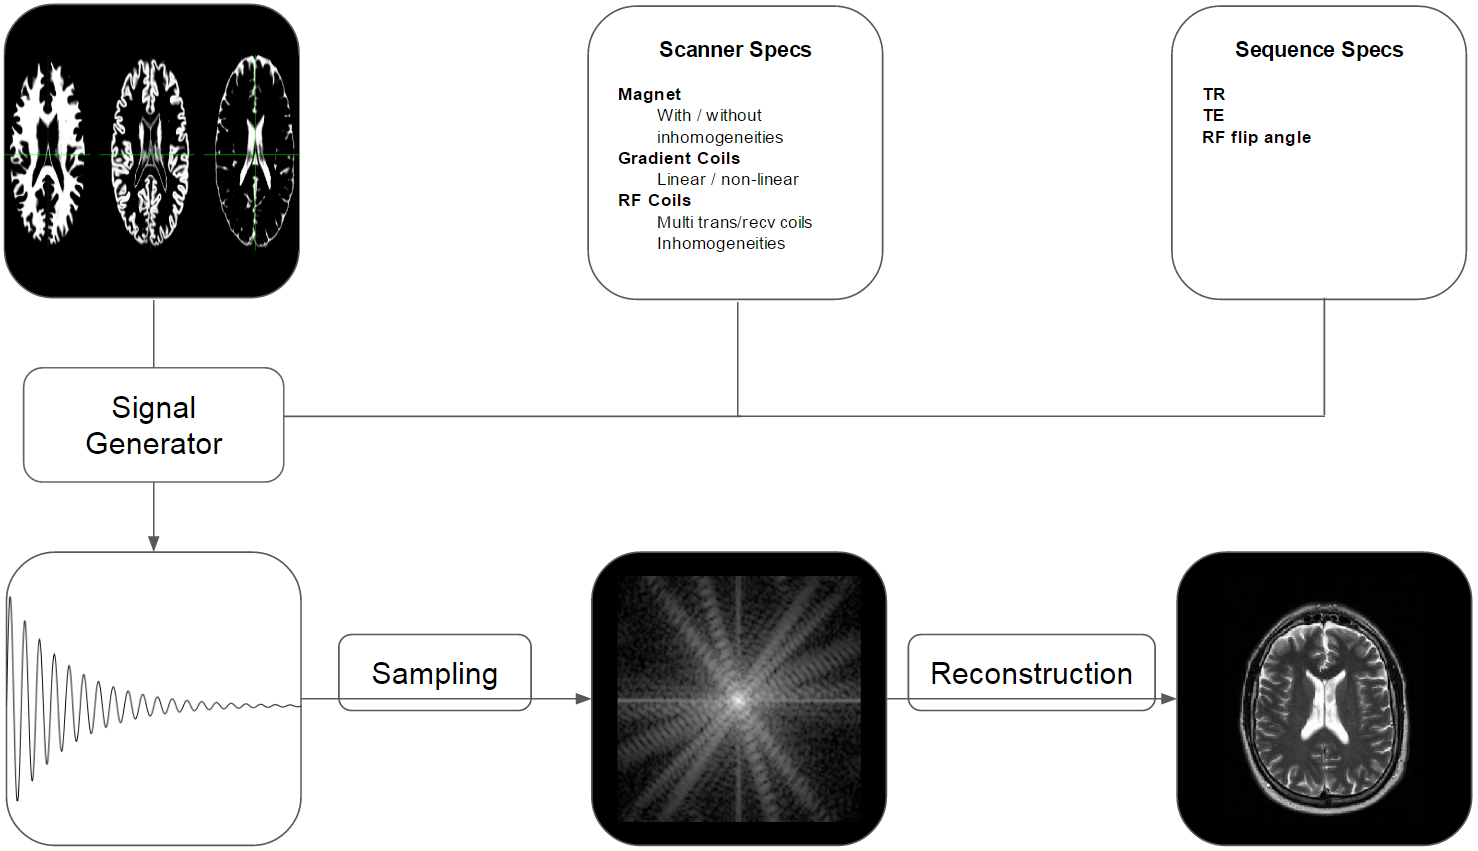
\includegraphics[width=1\textwidth,keepaspectratio]{mrisimscan}
    \caption{The MRI simulation pipeline}
    \label{fig:mrisimscan}
\end{figure}

As can be seen from Figure~\ref{fig:mrisimscan}, a new step was added for the signal creation. Without actual motion from precessing spins, the requirement now is to have a mathematical model that emulates that. Generally speaking, the \textit{Signal Generator} is a Bloch equation solver. 

It follows that, in order to develop a realistic MRI simulator a few criteria must be met. These requirements can be organized in the next categories:

% The next step is to create a taxonomy for the ideal MRI simulator. That being said, the main criteria and their divisions are: \\

\begin{itemize}
%%%% SAMPLE
\item{Sample}

\begin{enumerate}
    %% Geometry
    \item Geometric Representation
    % \begin{itemize}
    %     \item Shape
    %     \begin{itemize}
    %         \item Parametric form
    %         \item Non-parametric form
    %         \begin{itemize}
    %             \item Piecewise constant representation
    %             \item Lattice
    %         \end{itemize}
    %     \end{itemize}
        
    %     \item Resolution
        
    %     \item Relative positions of figures
    %     \begin{itemize}
    %         \item Euclidean representation
    %         \item Graph representation
    %     \end{itemize}
        
    % \end{itemize}
    
    %% Tissue Specific Parameters
    \item Tissue Specific Parameters
    % \begin{itemize}
    %     \item Proton Density
    %     \item $T_1$
    %     \item $T_2$
    %     \item $T_2^*$
    %     \item Chemical Shift
    %     \item Exchange Rates
    %     \item Susceptibility values
    % \end{itemize}
    
    %% Motion
    \item Motion
    % \begin{itemize}
    %     \item Rigid motion
    %     \item Non-rigid motion
    % \end{itemize}
\end{enumerate}


%%%% HARDWARE
\item{Hardware}
\begin{enumerate}
    %% Magnet
    \item Magnet
    % \begin{itemize}
    %     \item Strength
    %     \item Intrinsic inhomogeneities
    % \end{itemize}
    
    %% Gradients
    \item Gradient Coils
    % \begin{itemize}
    %     \item Slew Rates
    %     \item Gradient non-linearities
    % \end{itemize}
    
    %% RF Coils
    \item RF Coils
    % \begin{itemize}
    %     \item Type
    %     \item Number of Coils
    %     \item Intrinsic inhomogeneities
    % \end{itemize}
\end{enumerate}


%%%% SEQUENCE
\item{Sequence}
\begin{enumerate}
    \item Time constants
    % \begin{itemize}
    %     \item TR
    %     \item TE
    %     \item Gradients durations
    %     \item In-between gradients durations
    % \end{itemize}
    
    \item RF Pulse 
    % \begin{itemize}
    %     \item Shape
    %     \begin{itemize}
    %         \item Amplitude
    %         \item Carrier Frequency
    %         \item Initial Phase
    %     \end{itemize}
        
    %     \item Flip Angle
    % \end{itemize}
    
\end{enumerate}

%%%% SIGNAL GENERATOR
% \textbf{4. Signal Generator}
% \begin{itemize}
%     \item Solver
    
%     \item 
% \end{itemize}

%%%% RECONSTRUCTION
\item{Reconstruction}
% \begin{itemize}
    % \item By number of coils
    % \begin{itemize}
    %     \item Single Coil reconstruction
    %     \item Parallel Imaging reconstruction
    % \end{itemize}
% \end{itemize}

%%%% IMPLEMENTATION
% \item{Software Implementation}
\end{itemize}

Next, a survey of existing MRI simulators is being presented in terms of the previously stated criteria.

%%%%%%%%%%%%%%%%%%%%%%%%%%
\section{A survey of MRI Simulators}
%\textbf{Go in depth and explain how every simulator fits in the picture} \\

%%%%%%%%%%%%%%%%%%%
\subsection{Sample}
\subsubsection{Geometric Representation}

Real world objects can have different shapes and sizes. The question now is how these objects are represented geometrically. A first category that can be distinguished is related to how the shape of an object is defined digitally. That being said, the most commonly opted form is the \textit{piecewise constant representation}. This is because storing data in a structured, non-changing shape, where every position in the object is clearly defined and every neighbour is quickly found, is much more convenient for time requirements. 

Indeed, having defined a multi-dimensional matrix with each index representing a position in the object, the search and retrieval of information from the structure is faster than in a linked-list type of structure such as a mesh. Since the first realistic MR imaging simulators developed by Bittoun et al in 1984 \cite{Bittoun1984} who solved the Bloch equation for each point in a 1D object, followed by Summers et al \cite{Summers1986} and by Olsson et al \cite{Olsson1995} who went further, to 3D objects, this has become a standard for all simulators since. 

A different approach was taken by Kwan et al \cite{Kwan1999} who used tissue templates instead of finely grained collections of object points. This helped with computational speed as the magnetization vector was calculated only for the tissue types considered (such as WM, GM and CSF). The object of interest is still divided into cuboid elements and it contains the proportion of each tissue type present. The magnetization for a given voxel is then obtained by weighting the overall magnetization with the proportion of a certain tissue type and then summed over all templates. Although fast, it has many limitations such as the fact that it is not able to simulate certain artifacts caused by different object voxels experiencing different magnetic field inhomogeneities.

\subsubsection{Tissue Specific Parameters}
In terms of tissue specific parameters, ideally, an MRI simulator would have knowledge of every quantifiable element within the real tissue that is of interest to NMR. 

Generally speaking, the contrast in MR images is given by the proton density in that voxel and the tissue relaxation parameters, $T_1$ and $T_2$. That being said, most simulators to date rely on at least these 3 specifications. Bittoun et al \cite{Bittoun1984}, Olsson et al \cite{Olsson1995}, Petterson et al \cite{Petersson1993}, Hacklander et al \cite{Hacklander2005}, Kwan et al \cite{Kwan1999}, Benoit-Cattin et al \cite{Benoit-Cattin2005}, Xanthis et al \cite{Xanthis2014} and Jochimsen et al \cite{Jochimsen2004} require knowledge of PD, $T_1$ and $T_2$. Some other simulators such as the one developed by Drobnjak et al \cite{Drobnjak2006} use $T_2^*$ values instead of $T_2$ as their main focus is on functional MRI which takes into account the local magnetic field inhomogeneities. Others, such as the one created by Stocker et al \cite{Stocker2010} uses knowledge of both $T_2$ and $T_2^*$.

Another interesting aspect of the object being imaged is that of chemical shift as it produces inhomogeneities in the main magnetic field. This is a very important source of imaging artifacts and it is therefore a desired feature in a realistic simulator. Kwan et al \cite{Kwan1999}, Benoit-Cattin et al \cite{Benoit-Cattin2005}, Drobnjak et al \cite{Drobnjak2006}, Stocker et al \cite{Stocker2010}, Xanthis et al \cite{Xanthis2014}, Yoder et al \cite{Yoder2004} and Liu et al \cite{Liu2013} incorporate a $B_0$ inhomogeneity in their simulations.

In addition to these, for more sophisticated simulations, such as those required in \textit{magnetization transfer imaging}, knowledge of the various pools of spins is needed. Such an approach is presented by Liu et al \cite{Liu2016}. 

\subsubsection{Motion}
MRI is a very powerful imaging technique that provides great contrast between soft tissue types. Although one of the most used imaging modalities today, it is known to be prone to motion artifacts. Indeed, the quality of its images is affected by patient movements and pulsatile motion. For this, an accurate and realistic MRI simulator needs to take this into account. 

Clearly, this is a computationally intensive task as it requires calculations of magnetization vectors for all object voxels at each time point when motion is in place. Although it was not possible to simulate until more powerful computers arrived, it has now become one of the most desired traits in a simulator. Indeed, the still active, very powerful and realistic simulators treat this aspect within their software tool. Petterson et al \cite{Petersson1993} incorporates movement (or flow) in its k-space formalism approach without the possibility of simulating blurring artifacts. More sophisticated approaches such as those developed by Drobnjak et al \cite{Drobnjak2006} and Jochimsen et al \cite{Jochimsen2004} simulate rigid body motion during acquisition.

%%%%%%%%%%%%%%%%%%%
\subsection{Hardware}
\subsubsection{Magnet}
One of the key components of the MR scanner is the main magnet. It is an expensive piece of equipment used to generate the high fields required in MR imaging. Clinically, there are a few types of magnets available: closed bore (most widely used clinically as its strength range starts at 1T), open bore (these are permanent magnets with strengths that range from 0.2T and 0.7T) and dipolar electromagnets configurations (with a range of 0.5T to 1.2T) \cite{Morrow2000}. Regardless of their type, MR imaging requires perfect homogeneity in the field such that every part of the object being scanned experiences the expected field strength. In reality, parallel field lines are hard to obtain and so a scanner is equipped with shim coils which adjust the homogeneity of the field \cite{Romeo1984}.

That being said, a realistic MRI simulator should be equipped with at least 2 specifications: field strength and inhomogeneities in the main magnetic field. As the current aim of many MRI simulators is to provide a realistic, yet controlled way of generating MR images, all simulators available offer the possibility of field strength choice. In terms of intrinsic magnet inhomogeneities, there are no available simulators that model that, most of them focusing on susceptibility induced inhomogeneities as was discussed previously.

\subsubsection{Gradient Coils}
Gradient coils are part of the MR scanner hardware. Their purpose is to linearly vary the main magnetic field in a certain direction. Nearly all clinically available MR scanners have 3 types of gradient coils: the x-, y- and z- gradients, which alter the main magnetic field such that different parts of the object being imaged experience a slightly different field strength \cite{Hidalgo-Tobon2010}. This is at the heart of slice selection and frequency encoding, concepts which were discussed in the previous chapter. 

Turning to MRI simulation, it is obvious that the most important requirements that need to be part of the simulation pipeline are the gradient's strength and its direction. Besides this, other aspects are also essential. For example, one might want to model a non-linear variation in the gradients strength. This is available in the simulators developed by Benoit-Cattin et al \cite{Benoit-Cattin2005}, Stocker et al \cite{Stocker2010} and Liu et al \cite{Liu2013}. In addition, the time it takes for a gradient to reach its peak, called the \textit{rise time}, must be taken into consideration when realistic MRI simulation is desired. The most important reason for this is that the slew rates affect the minimum attainable TR or the spacing between spin echoes in fast imaging sequences. Among the available simulators, Drobnjak et al \cite{Drobnjak2006} and Xanthis et al \cite{Xanthis2014} allow for rise time configuration.

Furthermore, Jochimsen et al \cite{Jochimsen2004} provide a list of rotation matrices that can be used to move the gradient objects for diffusion MRI experiments. These matrices can also be user defined. In addition, Drobnjak et al \cite{Drobnjak2010} simulate time varying magnetic fields which are the main cause for eddy currents artifacts in diffusion MRI. 

\subsubsection{RF Coils}
The third main hardware component of an MR scanner is the RF coil. There are roughly two types of coils: volume and surface coils. The main difference between the two, besides their suggestive usage, is that the surface coils have a lower penetration depth than the volume ones. The surface coils are therefore able to retrieve better SNR for surface originating signals, while the volume coils provide a more homogeneous field. The spatially varying signal strength specific to surface coils is modelled by Stocker et al \cite{Stocker2010} and by Xanthis et al \cite{Xanthis2014} in their MRI simulators.

Now, as with any piece of electronic equipment, the scanner's RF coils are not perfect. It is therefore important when simulating the MRI pipeline to take inhomogeneities into consideration. Hacklander et al \cite{Hacklander2005} and Drobnjak et al \cite{Drobnjak2006} model noise and inhomogeneities in the receiving and transmitting coils. 

Moreover, multiple coils can be used simultaneously to transmit and receive signals. This is an available feature in the simulators developed by Jochimsen et al \cite{Jochimsen2004}, Liu et al \cite{Liu2014} and Stocker et al \cite{Stocker2010}.

%%%%%%%%%%%%%%%%%%%
\subsection{MRI Sequence}
The discussion so far was centered around the object being imaged and the MR scanner hardware. Another important part of the pipeline is the MRI sequence, which can be described as a set of radiofrequency pulses and changing magnetic field gradients, together with the order in which each of them should be performed and for how long. This "recipe" dictates the contrast in the image or the type of information available. For example, there are MRI sequences which can provide good anatomical contrast between different tissue types, while more sophisticated ones can be sensitized to flow or perfusion. Despite their large number, all of them rely on a set of parameters that can be modified in order to provide the best contrast for the requirements. 
%There are two main ways of categorizing the sequences: by the contrast provided (proton density, $T_1$, $T_2$ or $T_2^*$ weighted) or by their type (spin echo, gradient echo, etc).
In this section different MRI simulators will be investigated in terms of how they simulate the MR sequence.

\subsubsection{Time constants}
As stated before, all MRI sequences have a set of time related parameters that ultimately define the image contrast. That being said, one particularly popular approach in terms of simulation is to use the steady state solutions of the Bloch equations for some of the most clinically used sequences. For example, the spin-echo sequence can be described in terms of tissue specific parameters (proton density, $T_1$ and $T_2$) and sequence specific parameters such as: time to echo ($TE$) and time to repetition ($TR$). This approach aids the understanding of MR image contrast when the time constants are modified and is present in MRI simulations developed by Ortendahl et al \cite{Ortendahl1984}, Riederer et al \cite{Riederer1984}, Bobman et al \cite{Bobman1985}, Lufkin et al \cite{Lufkin1986}, Torheim et al \cite{Torheim1994}, Simmons et al \cite{Simmons1996} and Hacklander et al \cite{Hacklander2005}. 

Spin echo is not the only sequence that can be simulated this way. By adding a different time constant, the inversion time ($TI$), inversion-recovery sequences can be modelled. These are simulated by Ortendahl et al \cite{Ortendahl1984}, Torheim et al \cite{Torheim1994}, Simmons et al \cite{Simmons1996} and Torheim et al \cite{Torheim1994}. More sophisticated sequences such as saturation recovery or fast sequences such as FLASH or turbo spin echo, which require a flip angle smaller than $90^o$, are also modelled by Simmons et al \cite{Simmons1996} and Hacklander et al \cite{Hacklander2005}.

Turning to simulators which solve the Bloch equation for each object voxel and for each time point during the sequence, the time constants are generally the same. That being said, $TE$, $TR$ and $\alpha$ (flip angle) can be chosen in simulators developed by Benoit-Cattin et al \cite{Benoit-Cattin2005}, Stocker et al \cite{Stocker2010}, Drobnjak et al \cite{Drobnjak2006} and Kwan et al \cite{Kwan1999}. Moreover, predefined gradient echo and spin echo sequences are offer by Benoit-Cattin et al \cite{Benoit-Cattin2005} and Drobnjak et al \cite{Drobnjak2006}, while Jochimsen et al \cite{Jochimsen2004} offer, in addition, predefined PROPELLER-EPI, single-shot TrueFISP, multi-slice MDEFT and fully flow-compensated FLASH sequences.

Finally, Drobnjak et al \cite{Drobnjak2006} and Xanthis et al \cite{Xanthis2014} allow users to define their own pulse sequences. These take the form of an input file which contains the sequence parameters ($TE$, $TR$, field-of-view, flip angle, gradient strengths, etc) in a simulator dependent structure. Jochimsen et al \cite{Jochimsen2004} treats the pulse sequence creation from a object-oriented perspective, providing a class structure that can be easily extended with new functionality.

\subsubsection{RF Pulse}
RF pulses are an important part of the MRI scanning pipeline. They are key to image formation as they "tip" the net magnetization vector away from the main magnetic field allowing it to be eventually measured, sampled, stored into k-space and finally reconstructed into an image. Moreover, the carrier frequency of the RF pulses has to be equal to the Larmor frequency of the spins which reside in the slice of interest. This is one of the key components of slice selection.

It is therefore important to accurately simulate this behaviour. Although most simulators treat the RF pulse as an event which rotates the net magnetization vector through a flip angle, simulators developed by Xanthis et al \cite{Xanthis2014}, Jochimsen et al \cite{Jochimsen2004} and Liu et al \cite{Liu2013} offer different types of RF pulse models to be investigated. Among all, the common ones are: slice selective RF pulses (sinc and Gauss shaped), rectangular and adiabatic. Moreover, composite pulses, created by concatenating other available pulses, are offered by ODIN, the simulator developed by Jochimsen et al \cite{Jochimsen2004}.

%%%%%%%%%%%%%%%%%%%
\subsection{Reconstruction}
The steps described thus far included the object, the scanner hardware and the process of obtaining different types of contrasts in the final MR images. Next, signal arising from the excited tissue is collected during read out, sampled and then stored in a matrix form. The matrix form represents the image in the frequency domain and it is known as k-space. Performing an inverse Fourier transform allows the normal image to be reconstructed.

However, almost all clinical MRI scanners have recently incorporated more sophisticated reconstruction methods. One of these methods sits under the \textit{parallel imaging techniques} umbrella. These are a collection of reconstruction algorithms that can be used in conjunction with many existing imaging sequences to speed up scanning time. This can be achieved by skipping time-consuming phase-encoding steps and replacing the missing information with data coming from multiple receiver coils. 

Therefore, in order to achieve parallel imaging, two criteria must be met. First, instead of using one homogeneous volume coil, multiple rf surface coils distributed around the object of interest will be used. Each of these coils will have a particular sensitivity profile which is used to recover the missing information caused by skipping phase-encoding steps. Second, a reconstruction algorithm will reconstruct the final, unaliased, image by using the undersampled data and the individual coil sensitivities. 

Generally speaking, there are two types of reconstruction algorithms: the \textit{GRAPPA\footnote{GeneRalized Auto-calibrating Partially Parallel
Acquisition}-type} algorithms, which use the k-space undersampled data to reconstruct the images and the \textit{SENSE\footnote{SENSitivity Encoding}-type} algorithms, which use the aliased images to reconstruct the final artifact free images \cite{Deshmane2012}. There are also hybrid algorithms such as ASSET\footnote{Array Spatial Sensitivity Encoding Technique} and ARC\footnote{Auto-calibrating Reconstruction for Cartesian
Imaging}, both being implemented by GE\footnote{General Electric} scanners \cite{Yanasak2015}.

That being said, parallel imaging techniques should be addressed in simulation in order to develop new algorithms or to test the validity of the already existing ones. Moreover, besides being more cost effective than normal scans, pMRI can increase motion tolerance \cite{Yanasak2014}, making it a highly desirable feature. Although the simulators developed by Stocker et al \cite{Stocker2010}, Liu et al \cite{Liu2013} and Jochimsen et al \cite{Jochimsen2004} have multi-coil capabilities, only the latter one implements a pMRI reconstruction algorithm, more specifically, GRAPPA.

%%%%%%%%%%%%%%%%%%%%%%%%%%
\section{Active MRI Simulators}
This section will be concerned with the active MRI simulators. A description of each will be provided with the focus being on the most desirable features. In doing so, the key players will be identified and the MRI simulation stage will be set.

To begin with, patient movement is the most common cause for imaging artifacts. More often than not it is caused by involuntary actions such as blood flow, respiration or cardiac pulse, but it can also be caused by external factors such as mechanical vibrations. The resulting artifacts are called \textit{blurring} and \textit{ghosting} and are the result of phase and amplitude incongruities \cite{Pusey1986} between consecutive phase encoding steps. That being said, simulating motion artifacts is one of the most highly desirable MRI simulation features. Out of all active simulators, three of them simulate rigid-body motion during acquisition. These simulators are called POSSUM\footnote{Physics-Oriented Simulated Scanner for Understanding MRI} \cite{Drobnjak2006}, JEMRIS \cite{Stocker2010} and MRiLab \cite{Liu2013}.

Second, multicoil acquisition has become a standard in clinical MRI scanners as it is the first step towards faster scans when used in conjunction with parallel imaging reconstruction algorithms. That being said, it is an important feature to have in an MRI simulator. Of all active players, JEMRIS \cite{Stocker2010}, MRiLab \cite{Liu2013} and ODIN \cite{Jochimsen2004} provide multicoil acquisitions. Moreover, MRiLab \cite{Liu2013} offers the possibility to graphically construct the coil configuration or to load a user defined one.

Third, as MRI simulation is highly expensive computationally, most available simulators perform their experiments on cluster systems to reduce run time. In case one does not have a readily available cluster, a couple of the active simulators offer an alternative: GPU\footnote{Graphics processing unit} implementation. This is a more user friendly approach as GPUs are known to be highly powerful processing units and are most often than not available on personal computers. The MRI simulators which have this feature are MRISIMUL \cite{Xanthis2014} and MRiLab \cite{Liu2013}.

Finally, as previously stated, parallel reconstruction is a highly desirable trait. This is because all known MRI scanners clinically available implement one or two pMRI reconstruction algorithms. The only available simulator which performs GRAPPA reconstructions is ODIN \cite{Jochimsen2004}. 

These four described aspects of MRI simulation and the key players which implement them can be visually inspected in Figure~\ref{fig:activesim}, which also sets the stage for currently active MRI simulators.  

\begin{figure}[H]
    \centering
    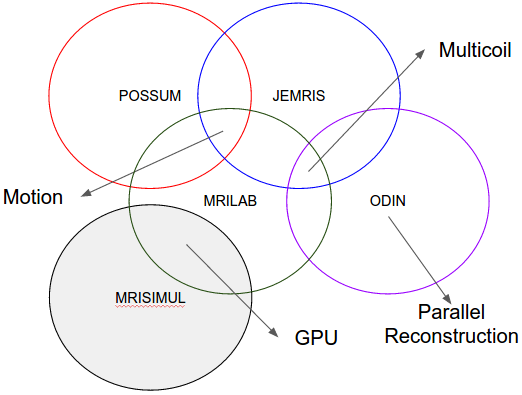
\includegraphics[width=\textwidth,keepaspectratio]{activesim}
    \caption{Active MRI Simulators}
    \label{fig:activesim}
\end{figure}

In conclusion, this section has presented the history of MRI simulation and its most important aspects in terms of a realistic MRI scan. The final subsection was focused on some of the most desirable features an MRI simulator should have. In doing so, it was found that parallel imaging techniques are not currently investigated by many of the aforementioned players. The purpose of this project is therefore to add parallel imaging capabilities to POSSUM, the \textit{Physics Oriented Simulated Scanner Utility for MRI} software tool developed by Drobnjak et al \cite{Drobnjak2006} and part of the FMRIB's software library\footnote{Created by the Analysis Group, FMRIB, Oxford, UK  \url{http://fsl.fmrib.ox.ac.uk/fsl/fslwiki/FSL}}.

